\chapter{Psalm 24}

\begin{figure}
  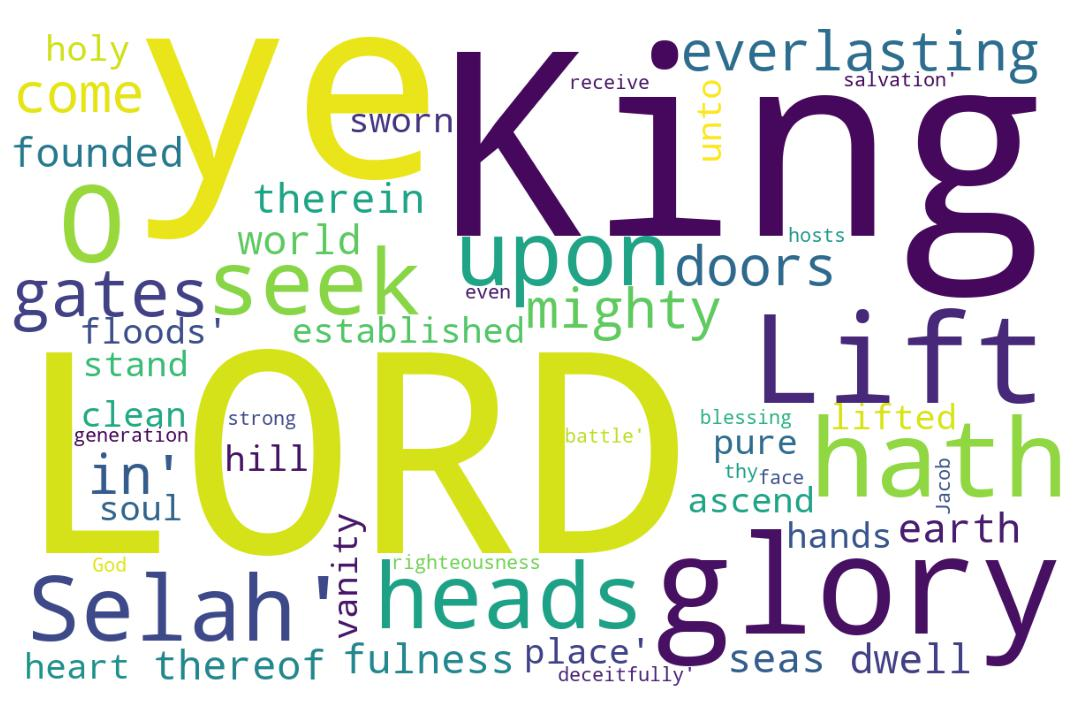
\includegraphics[width=\linewidth]{19OT-Psalms/Psalm24-WordCloud.jpg}
  \caption{Psalm 24 Word Cloud}
  \label{fig:Psalm 24 word Cloud}
\end{figure}


\marginpar{\scriptsize \centering \fcolorbox{bone}{lime}{\textbf{THE COMING KING}}\\ (Psalm 24:1-6) \begin{compactenum}[I.][8]
    \item \textbf{Going} to the King \index[scripture]{Psalms!Psa 024:03}(Psa 24:3)
    \item The \textbf{Godliness} of his Followers \index[scripture]{Psalms!Psa 024:04}(Psa 24:4)
    \item The \textbf{Grace} He Dispenses \index[scripture]{Psalms!Psa 024:05}(Psa 24:5)
    \item The \textbf{Generation} that seeks Him  \index[scripture]{Psalms!Psa 024:06}(Psa 24:6)
    \item A \textbf{Glimpse} of Him \index[scripture]{Psalms!Psa 024:07}\index[scripture]{John!John 18:01}(Psa 24:7, John 18:1)
    \item The \textbf{Gates} of New Jerusalem \index[scripture]{Psalms!Psa 024:07}\index[scripture]{Psalms!Psa 024:09}(Psa 24:7,9), pictured in \index[scripture]{Nehemiah!Neh 02}\index[scripture]{Nehemiah!Neh 003} (Neh 2-3)
    \item His \textbf{Glory} \index[scripture]{Psalms!Psa 024:07}\index[scripture]{Psalms!Psa 024:10}(Psa 24:7,10)
\end{compactenum}}

\marginpar{\scriptsize \centering \fcolorbox{bone}{yellow}{\textbf{REIGNING}}\\ (Psalm 24:1-6) \begin{compactenum}[I.][8]
    \item The \textbf{Hill} \index[scripture]{Psalms!Psa 024:03}(Psa 24:3)
    \item The \textbf{Holy Place} \index[scripture]{Psalms!Psa 024:03}(Psa 24:3)
    \item The \textbf{Heart} \index[scripture]{Psalms!Psa 024:04}(Psa 24:4)
    \item The \textbf{Hands} \index[scripture]{Psalms!Psa 024:04}(Psa 24:4)
    \item The \textbf{Heads} \index[scripture]{Psalms!Psa 024:07}\index[scripture]{Psalms!Psa 024:09}(Psa 24:7 9)
    \item The \textbf{Hosts} \index[scripture]{Psalms!Psa 024:10}(Psa 24:10)
\end{compactenum}}

\marginpar{\scriptsize \centering \fcolorbox{bone}{black}{\textbf{\textcolor[cmyk]{0,0,0,0}{PSALM 24}}}\\ (Psalm 24:1-6) \begin{compactenum}[I.][8]
    \item  \textbf{Existence} of the King \index[scripture]{Psalms!Psa 024:01-02}(Psa 24:1-2)
    \item  \textbf{Elligibility} for the Kingdom \index[scripture]{Psalms!Psa 024:05-06}(Psa 24:5-6)
    \item  \textbf{Entrance} of the King \index[scripture]{Psalms!Psa 024:07-09}(Psa 24:7-9)
    \item  \textbf{Excellence} of the King \index[scripture]{Psalms!Psa 024:10}(Psa 24:10)
\end{compactenum}}

\footnote{\textcolor[cmyk]{0.99998,1,0,0}{\hyperlink{TOC}{Return to end of Table of Contents.}}}\footnote{\href{https://www.audioverse.org/english/audiobibles/books/ENGKJV/O/Ps/1}{\textcolor[cmyk]{0.99998,1,0,0}{Psalms Audio}}}\textcolor[cmyk]{0.99998,1,0,0}{A Psalm of David.}\\
\\
\textcolor[cmyk]{0.99998,1,0,0}{The earth \emph{is} the LORD'S, and the fulness thereof; the world, and they that dwell therein.}\footnote{\textbf{1 Corinthians 10:26, 28} - For the earth is the Lord’s, and the fulness thereof. [28] But if any man say unto you, This is offered in sacrifice unto idols, eat not for his sake that shewed it, and for conscience sake: for the earth is the Lord’s, and the fulness thereof:}\footnote{\textbf{2 Corinthians 4:4} - In whom the god of this world hath blinded the minds of them which believe not, lest the light of the glorious gospel of Christ, who is the image of God, should shine unto them.}
[2] \textcolor[cmyk]{0.99998,1,0,0}{For he hath founded it upon the seas, and established it upon the floods.}
[3] \textcolor[cmyk]{0.99998,1,0,0}{Who shall \fcolorbox{bone}{lime}{ascend} into the hill of the LORD? or who shall stand in his holy place?}\footnote{\textbf{Psalm 2:6} - Yet have I set my king upon my holy hill of Zion.}\footnote{\textbf{Psalm 15:1-5} - LORD, who shall abide in thy tabernacle? who shall dwell in thy holy hill? [2] He that walketh uprightly, and worketh righteousness, and speaketh the truth in his heart. [3] He that backbiteth not with his tongue, nor doeth evil to his neighbour, nor taketh up a reproach against his neighbour. [4] In whose eyes a vile person is contemned; but he honoureth them that fear the LORD. He that sweareth to his own hurt, and changeth not. [5] He that putteth not out his money to usury, nor taketh reward against the innocent. He that doeth these things shall never be moved.}
[4] \textcolor[cmyk]{0.99998,1,0,0}{He that hath \fcolorbox{bone}{lime}{clean hands}, and a \fcolorbox{bone}{lime}{pure heart}; who hath \fcolorbox{bone}{lime}{not lifted up his soul} unto vanity, nor \fcolorbox{bone}{lime}{sworn deceitfully}.}
[5] \textcolor[cmyk]{0.99998,1,0,0}{He shall receive the \fcolorbox{bone}{lime}{blessing} from the LORD, and \fcolorbox{bone}{MYGOLD}{righteousness} from the God of his salvation.}
[6] \textcolor[cmyk]{0.99998,1,0,0}{This \emph{is} the generation of them that \fcolorbox{bone}{lime}{seek} him, that \fcolorbox{bone}{lime}{seek} thy face, O Jacob. Selah.}
[7] \textcolor[cmyk]{0.99998,1,0,0}{\fcolorbox{bone}{lime}{Lift up} your heads, O ye gates; and be ye lift up, ye everlasting \fcolorbox{bone}{lime}{doors}; and the King of \fcolorbox{bone}{lime}{glory} shall come in.}
[8] \textcolor[cmyk]{0.99998,1,0,0}{Who \emph{is} this King of \fcolorbox{bone}{lime}{glory}? The LORD strong and mighty, the LORD mighty in battle.}
[9] \textcolor[cmyk]{0.99998,1,0,0}{Lift up your heads, O ye gates; even lift \emph{them} up, ye everlasting \fcolorbox{bone}{lime}{doors}; and the King of glory shall come in.}
[10] \textcolor[cmyk]{0.99998,1,0,0}{Who is this King of \fcolorbox{bone}{lime}{glory}? The LORD of hosts, he \emph{is} the King of \fcolorbox{bone}{lime}{glory}. Selah.}